\documentclass[../../main.tex]{subfiles}
\begin{document}

{\bf [解]}
円の中心を$E(a,0)$とおいて $\angle CEA=\alpha,\ \angle BED=\beta$とする（$0<\alpha,\beta<\pi/2$）．
この様子を図に示す．

\begin{figure}[htb]
\begin{center}
\begin{tikzpicture}[scale=2, >=stealth]

  % --- パラメータ設定 (a != 0 の一般例) ---
  \def\aVal{0.4} % 中心 E の x 座標
  \def\rVal{1}   % 円の半径

  % 計算によって alpha, beta を求める (式(2)より)
  % cos(alpha) = 1/(2-a), cos(beta) = 1/(2+a)
  \pgfmathsetmacro{\alphaVal}{acos(1/(2-\aVal))}
  \pgfmathsetmacro{\betaVal}{acos(1/(2+\aVal))}

  % --- 座標定義 ---
  \coordinate (O) at (0,0);
  \coordinate (A) at (2,0);
  \coordinate (B) at (-2,0);
  \coordinate (E) at (\aVal,0);

  % 点 C, D の座標 (式(1)より)
  \coordinate (C) at ($ (E) + (\alphaVal:{\rVal}) $);
  \coordinate (D) at ($ (E) + ({180-\betaVal}:{\rVal}) $);

  % --- 描画 ---

  % 座標軸
  \draw[->, thin, gray] (-2.5, 0) -- (2.5, 0) node[right, black] {$x$};
  \draw[->, thin, gray] (0, -0.2) -- (0, 1.3) node[above, black] {$y$};
  \node[below left] at (O) {$O$};

  % 半円 (x-a)^2 + y^2 = 1, y>=0
  \draw[thick, blue!80!black] ($ (E) + (\rVal, 0) $) arc (0:180:\rVal);
  % 直径部分
  \draw[thin, gray] ($ (E) + (-\rVal, 0) $) -- ($ (E) + (\rVal, 0) $);

  % 接線 AC, BD
  \draw[thick, red!80!black] (A) -- ($ (A)!1.3!(C) $) node[above] {$\ell_C$};
  \draw[thick, red!80!black] (B) -- ($ (B)!1.3!(D) $) node[above] {$\ell_D$};

  % 半径 EC, ED (接線と直交)
  \draw[dashed, gray] (E) -- (C);
  \draw[dashed, gray] (E) -- (D);

  % --- 記号・ラベル ---

  % 点のプロット
  \fill[black] (A) circle (1pt) node[below] {$A(2,0)$};
  \fill[black] (B) circle (1pt) node[below] {$B(-2,0)$};
  \fill[black] (E) circle (1pt) node[below] {$E(a,0)$};
  \fill[black] (C) circle (1pt) node[above right] {$C$};
  \fill[black] (D) circle (1pt) node[above left] {$D$};

  % 垂線 C', D'
  \coordinate (Cprime) at (C |- O);
  \coordinate (Dprime) at (D |- O);
  \draw[dashed, gray] (C) -- (Cprime);
  \draw[dashed, gray] (D) -- (Dprime);
  % \fill[black] (Cprime) circle (0.8pt) node[below, yshift=-1pt] {$C'$};
  % \fill[black] (Dprime) circle (0.8pt) node[below, yshift=-1pt] {$D'$};

  % --- 角度 alpha, beta の表示 ---
  % 基準線用の見えない点
  \coordinate (E_east) at ($ (E) + (1,0) $);
  \coordinate (E_west) at ($ (E) + (-1,0) $);

  % Angle alpha
  \draw pic[draw, "$\alpha$", angle eccentricity=1.5, angle radius=15pt] {angle = E_east--E--C};
  % Angle beta
  \draw pic[draw, "$\beta$", angle eccentricity=1.5, angle radius=15pt] {angle = D--E--E_west};

  % 直角マーク (半径と接線)
  \draw[thin, gray] ($ (C)!5pt!(E) $) -- ($ ($ (C)!5pt!(E) $) + ($ (C)!5pt!(A) $)-(C) $) -- ($ (C)!5pt!(A) $);
  \draw[thin, gray] ($ (D)!5pt!(E) $) -- ($ ($ (D)!5pt!(E) $) + ($ (D)!5pt!(B) $)-(D) $) -- ($ (D)!5pt!(B) $);

\end{tikzpicture}
\caption{題意の状況}
\end{center}
\end{figure}


この時$C, D$の座標は
\begin{align}
\begin{cases}
C(a+\cos\alpha,\sin\alpha) \\
D(a-\cos\beta,\sin\beta) 
\end{cases} \label{eq:1}
\end{align}
だから$C,D$での円の接線$\ell_C,\ell_D$は
\begin{align}
\begin{cases}
\ell_C: (\cos\alpha)(x-a)+\sin\alpha\cdot y&=1 \\
\ell_D: (-\cos\beta)(x-a)+\sin\beta\cdot y&=1 
\end{cases}
\end{align}
と書ける．
これらがそれぞれ$A(2,0),B(-2,0)$を通るから$\ell_C,\ell_D$の方程式に代入して
\begin{align}
\cos\alpha=\dfrac{1}{2-a}, \qquad \cos\beta=\dfrac{1}{2+a} \quad\cdots\text{②} \label{eq:2}
\end{align}
である．

\begin{figure}[htb]
\begin{center}
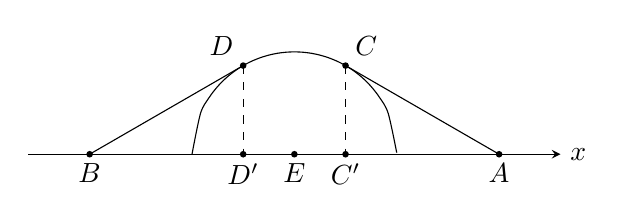
\begin{tikzpicture}[scale=1.3, >=stealth]
  % 座標軸
  \draw[->] (-2.6,0) -- (2.6,0) node[right] {$x$};
  % 半円 (x-a)^2+y^2=1, y>=0 (a=0の対称な場合を例示)
  \draw[domain=-1:1, smooth] plot ({\x},{sqrt(1-\x*\x)});
  % 接線 BD, AC (a=0の時 cos alpha=cos beta=1/2 より alpha=beta=60度)
  \draw (-2,0) -- (-0.5,0.8660);
  \draw (2,0) -- (0.5,0.8660);
  \fill (0,0) circle (0.92pt) node[below] {$E$};
  \fill (-2,0) circle (0.92pt) node[below] {$B$};
  \fill (2,0) circle (0.92pt) node[below] {$A$};
  \fill (-0.5,0.8660) circle (0.92pt) node[above left] {$D$};
  \fill (0.5,0.8660) circle (0.92pt) node[above right] {$C$};
  \fill (-0.5,0) circle (0.92pt) node[below] {$D'$};
  \fill (0.5,0) circle (0.92pt) node[below] {$C'$};
  \draw[dashed] (-0.5,0.8660) -- (-0.5,0);
  \draw[dashed] (0.5,0.8660) -- (0.5,0);
  % 半円の直径部分 (回転体の底面)
  \draw (-1,0) -- (1,0);
\end{tikzpicture}
\end{center}
\caption{点$A$，$B$，$C$，$D$，$E$の位置関係}
\end{figure}

題意の回転体の体積を$V(a)$とする．この回転体は$y$座標の小さい方から順に，線分$BD$を回転させた円錐，$DC$間の弧を回転させた部分，線分$AC$を回転させた円錐の3つの部分から成る．

\begin{align}
  V(a) &=
  % --- 1つ目の円錐 ---
  \left( \text{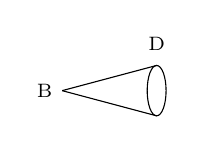
\begin{tikzpicture}[baseline={(0,0.1)}, scale=0.8, >=stealth]
    % 頂点 B
    \node[anchor=east, font=\scriptsize] at (0,0.4) {B};
    % 円錐の輪郭
    \draw (0,0.4) -- (1.5,0);
    \draw (0,0.4) -- (1.5,0.8);
    % 底面の円（楕円）
    \draw (1.5,0.4) ellipse (0.15 and 0.4);
    % 点D
    \node[anchor=south, font=\scriptsize, yshift=2pt] at (1.5,0.8) {D};
  \end{tikzpicture}} \right)
  +
  % --- 2つ目の回転体 ---
  \left( \text{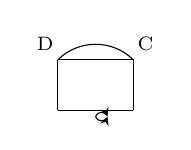
\begin{tikzpicture}[baseline={(0,0.1)}, scale=0.8, >=stealth]
    % 軸
    \draw (0,0) -- (1.2,0);
    \draw (0,0.8) -- (1.2,0.8);
    \draw (0,0) -- (0,0.8);
    \draw (1.2,0) -- (1.2,0.8);
    % 上の曲線
    \draw (0,0.8) to[out=45, in=135] (1.2,0.8);
    % 回転矢印
    \draw[->] (0.6, -0.1) arc (200:340:0.1);
    \draw[->] (0.6, -0.1) arc (160:20:0.1);
    % ラベル D, C
    \node[anchor=south east, font=\scriptsize, xshift=2pt] at (0,0.8) {D};
    \node[anchor=south west, font=\scriptsize, xshift=-2pt] at (1.2,0.8) {C};
  \end{tikzpicture}} \right)
  +
  % --- 3つ目の円錐 ---
  \left( \text{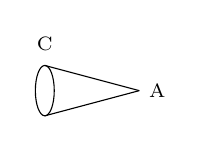
\begin{tikzpicture}[baseline={(0,0.1)}, scale=0.8, >=stealth]
    % 頂点 A
    \node[anchor=west, font=\scriptsize] at (1.5,0.4) {A};
    % 円錐の輪郭
    \draw (1.5,0.4) -- (0,0);
    \draw (1.5,0.4) -- (0,0.8);
    % 底面の円（楕円）と点C
    \draw (0,0.4) ellipse (0.15 and 0.4);
    \node[anchor=south, font=\scriptsize, yshift=2pt] at (0,0.8) {C};
  \end{tikzpicture}} \right) \label{eq:3}
\end{align}

各項を個別に計算しよう．わかりやすさのために$C,D$から$x$軸におろした垂線の足を$C',D'$とおくと\cref{eq:1}より
\begin{align}
\begin{cases}
 |DD'| &= \sin\beta \\
 |D'B| &= a-\cos\beta+2 \\
 |CC'| &= \sin\alpha \\
 |C'A| &= 2-a-\cos\alpha 
\end{cases}
\end{align}
である．$\triangle_D$は底面の半径$|DD'|$高さ$D'B$の円錐であって，$\triangle_C$は底面の半径$|CC'|$高さ$|AC'|$の円錐であるから\cref{eq:2}にも注意して
\begin{align}
  \left( \text{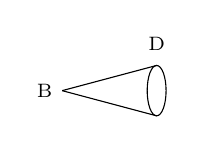
\begin{tikzpicture}[baseline={(0,0.1)}, scale=0.8, >=stealth]
    % 頂点 B
    \node[anchor=east, font=\scriptsize] at (0,0.4) {B};
    % 円錐の輪郭
    \draw (0,0.4) -- (1.5,0);
    \draw (0,0.4) -- (1.5,0.8);
    % 底面の円（楕円）
    \draw (1.5,0.4) ellipse (0.15 and 0.4);
    % 点D
    \node[anchor=south, font=\scriptsize, yshift=2pt] at (1.5,0.8) {D};
  \end{tikzpicture}} \right)
   &=\dfrac{1}{3}\left(\pi|DD'|^2\right)\cdot |D'B| \\
   &=\dfrac{1}{3}\cdot(\pi\sin^2\beta)\cdot(a-\cos\beta+2) \\
   &=\dfrac{\pi}{3}\left(1-\left(\dfrac{1}{2+a}\right)^2\right)\left(a+2-\dfrac{1}{2+a}\right) \quad(\because\text{\cref{eq:2}}) \\
   &=\dfrac{\pi}{3}\cdot\dfrac{\{(2+a)^2-1\}^2}{(2+a)^3} \label{eq:4}\\
  \left( \text{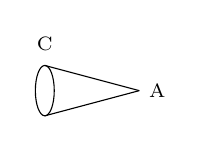
\begin{tikzpicture}[baseline={(0,0.1)}, scale=0.8, >=stealth]
    % 頂点 A
    \node[anchor=west, font=\scriptsize] at (1.5,0.4) {A};
    % 円錐の輪郭
    \draw (1.5,0.4) -- (0,0);
    \draw (1.5,0.4) -- (0,0.8);
    % 底面の円（楕円）と点C
    \draw (0,0.4) ellipse (0.15 and 0.4);
    \node[anchor=south, font=\scriptsize, yshift=2pt] at (0,0.8) {C};
  \end{tikzpicture}} \right) 
   &=\dfrac{1}{3}\left(\pi|CC'|^2\right)\cdot |C'A| \\
   &=\dfrac{1}{3}(\pi\sin^2\alpha)(2-a-\cos\alpha) \\
   &=\dfrac{\pi}{3}\left(1-\left(\dfrac{1}{2-a}\right)^2\right)\left(2-a-\dfrac{1}{2-a}\right) \quad(\because\text{\cref{eq:2}}) \\
   &=\dfrac{\pi}{3}\cdot\dfrac{\{(2-a)^2-1\}^2}{(2-a)^3} \label{eq:5}
\end{align}
である．
最後に円弧$CD$の回転体部分は
\begin{align}
  \left( \text{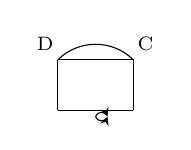
\begin{tikzpicture}[baseline={(0,0.1)}, scale=0.8, >=stealth]
    % 軸
    \draw (0,0) -- (1.2,0);
    \draw (0,0.8) -- (1.2,0.8);
    \draw (0,0) -- (0,0.8);
    \draw (1.2,0) -- (1.2,0.8);
    % 上の曲線
    \draw (0,0.8) to[out=45, in=135] (1.2,0.8);
    % 回転矢印
    \draw[->] (0.6, -0.1) arc (200:340:0.1);
    \draw[->] (0.6, -0.1) arc (160:20:0.1);
    % ラベル D, C
    \node[anchor=south east, font=\scriptsize, xshift=2pt] at (0,0.8) {D};
    \node[anchor=south west, font=\scriptsize, xshift=-2pt] at (1.2,0.8) {C};
  \end{tikzpicture}} \right)
  &=\pi\int_{a-\cos\beta}^{a+\cos\alpha}\{1-(x-a)^2\}dx \\
  &=\pi\int_{-\cos\beta}^{\cos\alpha}(1-x^2)dx \\
  &=\pi\left[x-\dfrac{1}{3}x^3\right]_{-\frac{1}{2+a}}^{\frac{1}{2-a}} \quad(\because\text{\cref{eq:2}}) \\
  &=\pi\left\{\left(\dfrac{1}{2-a}+\dfrac{1}{2+a}\right)-\dfrac{1}{3}\left(\left(\dfrac{1}{2-a}\right)^3+\left(\dfrac{1}{2+a}\right)^3\right)\right\} \label{eq:6}
\end{align}
である．

以上\cref{eq:4,eq:5,eq:6}を\cref{eq:3}に代入して
\begin{align}
\begin{split}
V(a)
  &=\dfrac{\pi}{3}\left[\dfrac{\{(2-a)^2-1\}^2}{(2-a)^3}+\dfrac{\{(2+a)^2-1\}^2}{(2+a)^3}-\dfrac{1}{(2-a)^3}-\dfrac{1}{(2+a)^3}\right]+\pi\left[\dfrac{1}{2+a}+\dfrac{1}{2-a}\right] \\
  &=\dfrac{\pi}{3}\left[\dfrac{(a+3)^2(a^2+4a+2)}{(2+a)^3}+\dfrac{(a-3)^2(a^2-4a+2)}{(2-a)^3}\right]+\pi\left[\dfrac{1}{2+a}+\dfrac{1}{2-a}\right] \\
  &=\dfrac{\pi}{3}\left[\dfrac{a^3+4a+2+3}{2+a}+\dfrac{a^3-4a+2+3}{2-a}\right] \\
  &=\dfrac{\pi}{3}\left[a+2+\dfrac{1}{2+a}+2-a+\dfrac{1}{2-a}\right] \\
  &=\dfrac{\pi}{3}\left(4+\dfrac{1}{2+a}+\dfrac{1}{2-a}\right)
\end{split}
\end{align}
が求める体積である．

\newpage

\end{document}
